% ~~~~~~~~~~~~~~~~~~~~~~~ Preamble ~~~~~~~~~~~~~~~~~~~~~~~
\documentclass{article}

\usepackage{amsmath}
\usepackage{amssymb}
\usepackage{amsthm}
\usepackage{bpextra}
\usepackage{enumitem}
\usepackage{float}
\usepackage[hidelinks]{hyperref}
\usepackage{latexsym}
\usepackage{natbib}
\usepackage{pdfpages}
\usepackage{subcaption}
\usepackage{tikz}
\usepackage{tkz-berge}
\usepackage{titlesec}
\usepackage{varwidth}

% tikz things
\usetikzlibrary{petri, topaths, positioning, decorations.pathmorphing}

% natbib source
\bibliographystyle{agsm}
\renewcommand{\bibsection}{}

\pgfarrowsdeclare{arr}{arr}{
  \setlength{\arrowsize}{2\pgflinewidth}
  \addtolength{\arrowsize}{.5\pgflinewidth}
  \pgfarrowsrightextend{-1\arrowsize}
  \pgfarrowsleftextend{1\arrowsize}
}{
  \setlength{\arrowsize}{2\pgflinewidth}
  \addtolength{\arrowsize}{.5\pgflinewidth}
  \pgfpathmoveto{\pgfpoint{-5\arrowsize}{4\arrowsize}}
  \pgfpathlineto{\pgfpointorigin}
  \pgfpathlineto{\pgfpoint{-5\arrowsize}{-4\arrowsize}}
  \pgfusepathqstroke
}

\newcommand{\drawsquig}{\draw[-arr,
line join=round,
decorate, decoration={
    zigzag,
    segment length=4,
    amplitude=.9,post=lineto,
    post length=2pt
}]}

\newcommand\vc[1]{\vcenter{\hbox{#1}}}

\newcommand\atom[1]{%
 \ifx#11a\else%
 \ifx#12b\else%
 \ifx#13c\else%
 \fi\fi\fi
}

\newcommand\0{0}
\newcommand\1{1}
\newcommand\+{+}
\renewcommand\*{\times}

\newcommand{\tightplus}{\!+\!}
\newcommand{\tighttimes}{\!\*\!}
\newcommand\subs[1]{\mathsf{|#1|}}

\tikzstyle{tok}=[circle,inner sep=0pt,minimum size=4pt,outer sep=1pt]
\tikzstyle{src}=[black,text height=1ex,text depth=0ex,rotate=90]
\tikzstyle{tgt}=[black,text height=1ex,text depth=0ex]%,rotate=-45]
\tikzstyle{for}=[text height=1.5ex,text depth=.25ex]
\tikzstyle{jmp}=[->,line width=1pt,cap=round,gray]
\tikzstyle{jmp1}=[jmp]
\tikzstyle{jmp2}=[jmp,red]

\tikzstyle{tokB}=[fill,tok]
\tikzstyle{tokG}=[fill,tok,gray]
\tikzstyle{tokR}=[fill,tok,red]
\tikzstyle{tokRed}=[fill,tok,red]
\tikzstyle{tokBlue}=[fill,tok,blue]
\tikzstyle{tokGreen}=[fill,tok,darkgreen]
\tikzstyle{tokF}=[draw,thick,gray,circle,inner sep=0pt, minimum size=7pt]

\tikzstyle{matrix}=[x=-5mm,y=5mm,rotate=-90]


\titlespacing{\section}{0pt}{12pt plus 4pt minus 2pt}{0pt plus 2pt minus 2pt}
%\titleformat{\section}
%  {\normalfont\scshape}{\thesection}{1em}{}

% no paragraph indent
\setlength{\parindent}{0em}
\setlength{\parskip}{1em}
%\setlength{\columnsep}{2em}

% delta-equals (unused)
\def\deltaeq{\mathrel{\ensurestackMath{\stackon[1pt]{=}{\scriptstyle\Delta}}}}
% define-equals
\def\defeq{::=}
% set-to-equals
\def\seteq{:=}

% scalable proof tree
\newenvironment{scprooftree}[1]%
  {\gdef\scalefactor{#1}\begin{center}\proofSkipAmount \leavevmode}%
  {\scalebox{\scalefactor}{\DisplayProof}\proofSkipAmount \end{center} }


% indented definitions, lemmas etc
\makeatletter
\newtheoremstyle{indented}
    {15pt}% space before
    {5pt}% space after
    {\addtolength{\@totalleftmargin}{0em}
     \addtolength{\linewidth}{-0em}
     \parshape 1 0em \linewidth}% body font
    {-0em}% indent
    {\bfseries}% header font
    {.}% punctuation
    {\newline}% after theorem header
    {}% header specification (empty for default)
\makeatother


% theorems with global counter
\theoremstyle{indented}
\newtheorem{sec-ctr}{???}[section]
\newtheorem{definition}[sec-ctr]{Definition}
\newtheorem*{definition*}{Definition}
\newtheorem{proposition}[sec-ctr]{Proposition}
\newtheorem*{proposition*}{Proposition}
\newtheorem{lemma}[sec-ctr]{Lemma}
\newtheorem*{lemma*}{Lemma}
\newtheorem{example}[sec-ctr]{Example}
\newtheorem*{example*}{Example}
\newtheorem*{examples}{Examples}
\newtheorem{corollary}[sec-ctr]{Corollary}
\newtheorem*{corollary*}{Corollary}
\newtheorem{remark}[sec-ctr]{Remark}
\newtheorem*{remark*}{Remark}
\newtheorem*{remarks}{Remarks}


\newcommand\dual{\overline}

\title{From Additive to Classical Proof Search}
\author{Adam Lassiter\\Department of Computer Science\\University of Bath \and Willem Heijltjes\\Department of Computer Science\\University of Bath}
\date{}

\begin{document}
    {\let\newpage\relax\maketitle}

    \maketitle


    \section*{Introduction}
        Building on the work done by \citet{petri-nets}, we investigate proof search in classical logic through Additive Linear Logic (ALL).
        The process we investigate, called \textit{coalescence}, is a top-down proof search from axiom links down to the conclusion.
        This method is promising as it boasts great efficiency for ALL proof search and has a natural transformation to sequent calculus proofs.



    \section*{Additive Linear Logic}
        ALL is the fragment of linear logic that concerns sum $(+)$ and product $(\*)$, with their units $0$ and $1$. A \emph{formula} of ALL is constructed:
        \begin{equation*}
            A, B, C \quad \defeq \quad 0 \mid 1 \mid a \mid \dual a \mid A + B \mid A \* B
        \end{equation*}
        We write $\subs A$ for the set of subformula occurrences of $A$ (we distinguish both occurrences of $a$ in $a\*a$).

        A sequent for ALL is a pair $\vdash A,B$, and a sequent calculus for ALL is given by the following rules (where the symmetric rules operating on the second element of the pair $\vdash A,B$ are omitted):
        \begin{figure}[H]
            \centering
            \begin{minipage}{0.3\linewidth}
                \begin{prooftree}
                    \AxiomC{~}
                    \RightLabel{$\mathsf{ax}$}
                    \UnaryInfC{$\vdash a,\dual a$}
                \end{prooftree}
            \end{minipage}
            \begin{minipage}{0.3\linewidth}
                \begin{prooftree}
                    \AxiomC{~}
                    \RightLabel{$\1$}
                    \UnaryInfC{$\vdash \1,A$}
                \end{prooftree}
            \end{minipage}
            \begin{minipage}{0.3\linewidth}
                \begin{prooftree}
                    \AxiomC{$\vdash A,C$}
                    \RightLabel{$\+_1$}
                    \UnaryInfC{$\vdash A\+B,C$}
                \end{prooftree}
            \end{minipage}


            \begin{minipage}{0.4\linewidth}
                \begin{prooftree}
                    \AxiomC{$\vdash B,C$}
                    \RightLabel{$\+_2$}
                    \UnaryInfC{$\vdash A\+B,C$}
                \end{prooftree}
            \end{minipage}
            \begin{minipage}{0.4\linewidth}
                \begin{prooftree}
                    \AxiomC{$\vdash A,C$}
                    \AxiomC{$\vdash B,C$}
                    \RightLabel{$\*$}
                    \BinaryInfC{$\vdash A\*B,C$}
                \end{prooftree}
            \end{minipage}
        \end{figure}


    \section*{Coalescence Proof Search}
        Naively searching for a sequent proof, starting from a given conclusion, is exponential: the additive conjunction rule $(\*)$ duplicates its context $C$, and reciprocated duplication between both formulas in the sequent creates exponential growth.

        A more efficient algorithm, first observed by Galmiche \&\ Marion~\cite{..} and later by \citet{petri-nets}, is given by placing proof search for a sequent $\vdash A,B$ in the product space $\subs A\* \subs B$.
        This set contains all \emph{sub-sequents} of $\vdash A,B$ that might occur in a sequent proof of $\vdash A,B$, without redundancy.
        We represent $\subs A\* \subs B$ by a grid, e.g.\ that for $\vdash \dual a\+(\dual b\+\dual c),(a\* b)\*c$ is below:
        \[
            \vc{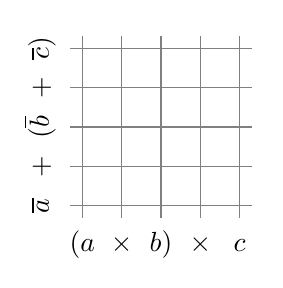
\begin{tikzpicture}[matrix]
                \foreach \x/\a in {1/\dual{\atom1}, 2/\+, 3/(\dual{\atom2}, 4/\+, 5/\dual{\atom3})}%
                    \draw[gray] (\x,0) node[src] {$\a$} (\x,.7) -- (\x,5.3);
                \foreach \y/\b in {1/(\atom1, 2/\*, 3/\atom2), 4/\*, 5/\atom3}%
                    \draw[gray] (0,\y) node[tgt] {$\b$} (.7,\y) -- (5.3,\y);
            \end{tikzpicture}}
            \quad\rightsquigarrow\quad
            \vc{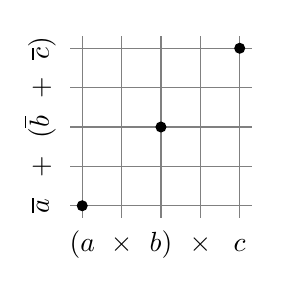
\begin{tikzpicture}[matrix]
                \foreach \x/\a in {1/\dual{\atom1}, 2/\+, 3/(\dual{\atom2}, 4/\+, 5/\dual{\atom3})}%
                    \draw[gray] (\x,0) node[src] {$\a$} (\x,.7) -- (\x,5.3);
                \foreach \y/\b in {1/(\atom1, 2/\*, 3/\atom2), 4/\*, 5/\atom3}%
                    \draw[gray] (0,\y) node[tgt] {$\b$} (.7,\y) -- (5.3,\y);
                \foreach \p/\n in { {1,1}/a1, {3,3}/b1, {5,5}/c1} \node[tokB] (\n) at (\p) {};
            \end{tikzpicture}}
        \]

        The \emph{coalescence proof search} algorithm for ALL is then as follows. We place tokens on this grid to indicate a sub-sequent is provable. Initially, we place tokens on each position $(\dual a,a)$, $(\1,A)$, and $(A,\1)$, as shown above right for our example. Then, we apply the following local rules (and the symmetric variants).
        \begin{itemize}
                \item Place a token on $(A\+B,C)$ if $(A,C)$ has a token.
                \item Place a token on $(A\+B,C)$ if $(B,C)$ has a token.
                \item Place a token on $(A\*B,C)$ if $(A,C)$ and $(B,C)$ have a token.
        \end{itemize}
        We illustrate these graphically as follows; note, though, that the \emph{neighbours} of a position in the grid are given by the subformula relation, and not by adjacency in the plane.
        \[
            \def\dual{}
            \begin{array}{ccc}
                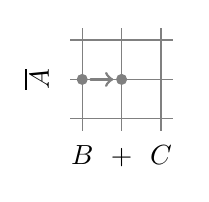
\begin{tikzpicture}[matrix]
                    \foreach \i/\a in {1/{}, 2/\dual A, 3/{}}
                        {\draw[gray] (\i,0) node[src] {$\a$} (\i,.7) -- (\i,3.3);}
                    \foreach \j/\b in {1/B, 2/\+, 3/C}
                        {\draw[gray] (0,\j) node[tgt] {$\b$} (.7,\j) -- (3.3,\j);}
                    \node[tokG] (a) at (2,1) {};
                    \node[tokG] (c) at (2,2) {};
                    \draw[jmp1] (a) to (c);
                \end{tikzpicture}
                &
                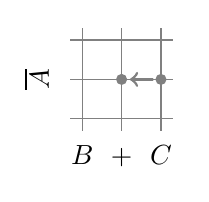
\begin{tikzpicture}[matrix]
                    \foreach \i/\a in {1/{}, 2/\dual A, 3/{}}
                        {\draw[gray] (\i,0) node[src] {$\a$} (\i,.7) -- (\i,3.3);}
                    \foreach \j/\b in {1/B, 2/\+, 3/C}
                        {\draw[gray] (0,\j) node[tgt] {$\b$} (.7,\j) -- (3.3,\j);}
                    \node[tokG] (b) at (2,3) {};
                    \node[tokG] (c) at (2,2) {};
                    \draw[jmp1] (b) to (c);
                \end{tikzpicture}
                &
                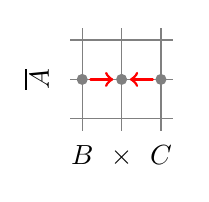
\begin{tikzpicture}[matrix]
                  \foreach \i/\a in {1/{}, 2/\dual A, 3/{}}
                    {\draw[gray] (\i,0) node[src] {$\a$} (\i,.7) -- (\i,3.3);}
                  \foreach \j/\b in {1/B, 2/\*, 3/C}
                    {\draw[gray] (0,\j) node[tgt] {$\b$} (.7,\j) -- (3.3,\j);}
                  \node[tokG] (a) at (2,1) {};
                  \node[tokG] (b) at (2,3) {};
                  \node[tokG] (c) at (2,2) {};
                  \draw[jmp2] (a) to (c);
                  \draw[jmp2] (b) to (c);
                \end{tikzpicture}
                \\ \\
                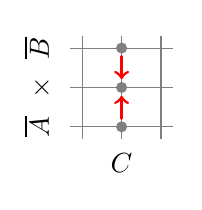
\begin{tikzpicture}[matrix]
                    \foreach \i/\a in {1/\dual A, 2/\*, 3/\dual B}
                        {\draw[gray] (\i,0) node[src] {$\a$} (\i,.7) -- (\i,3.3);}
                    \foreach \j/\b in {1/{}, 2/C, 3/{}}
                        {\draw[gray] (0,\j) node[tgt] {$\b$} (.7,\j) -- (3.3,\j);}
                    \node[tokG] (a) at (1,2) {};
                    \node[tokG] (b) at (3,2) {};
                    \node[tokG] (c) at (2,2) {};
                    \draw[jmp2] (a) to (c);
                    \draw[jmp2] (b) to (c);
                \end{tikzpicture}
                &
                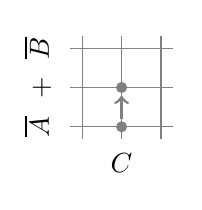
\begin{tikzpicture}[matrix]
                    \foreach \i/\a in {1/\dual A, 2/\+, 3/\dual B}
                        {\draw[gray] (\i,0) node[src] {$\a$} (\i,.7) -- (\i,3.3);}
                    \foreach \j/\b in {1/{}, 2/C, 3/{}}
                        {\draw[gray] (0,\j) node[tgt] {$\b$} (.7,\j) -- (3.3,\j);}
                    \node[tokG] (a) at (1,2) {};
                    \node[tokG] (c) at (2,2) {};
                    \draw[jmp1] (a) to (c);
                \end{tikzpicture}
                &
                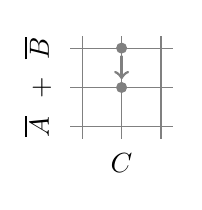
\begin{tikzpicture}[matrix]
                    \foreach \i/\a in {1/\dual A, 2/\+, 3/\dual B}
                        {\draw[gray] (\i,0) node[src] {$\a$} (\i,.7) -- (\i,3.3);}
                    \foreach \j/\b in {1/{}, 2/C, 3/{}}
                        {\draw[gray] (0,\j) node[tgt] {$\b$} (.7,\j) -- (3.3,\j);}
                    \node[tokG] (b) at (3,2) {};
                    \node[tokG] (c) at (2,2) {};
                    \draw[jmp1] (b) to (c);
                \end{tikzpicture}
            \end{array}
        \]
        Observe also that the initial token placement and the propagation rules corresponds directly to the axioms respectively the rules of the sequent rules for ALL.

        Finally, if the root position $(A,B)$ for $\vdash A,B$ has a token, we succeed; otherwise, if no more tokens can be placed we fail. For our example, we get the following trace:
        \[
            \vc{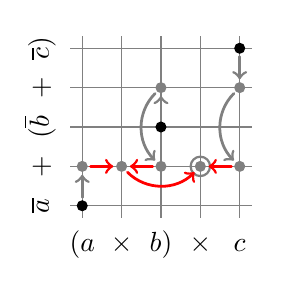
\begin{tikzpicture}[matrix]
                \foreach \x/\a in {1/\dual{\atom1}, 2/\+, 3/(\dual{\atom2}, 4/\+, 5/\dual{\atom3})}%
                    \draw[gray] (\x,0) node[src] {$\a$} (\x,.7) -- (\x,5.3);
                \foreach \y/\b in {1/(\atom1, 2/\*, 3/\atom2), 4/\*, 5/\atom3}%
                    \draw[gray] (0,\y) node[tgt] {$\b$} (.7,\y) -- (5.3,\y);
                \foreach \p/\n in {
                    {2,1}/a2, {2,2}/ab,
                    {4,3}/b2, {2,3}/b3,
                    {4,5}/c2, {2,5}/c3%
                } \node[tokG] (\n) at (\p) {};
                \node[tokG] (abc) at (2,4) {};
                \node[circle,draw,gray,thick,inner sep=0pt,minimum size=7pt] at (2,4) {};
                \foreach \p/\n in { {1,1}/a1, {3,3}/b1, {5,5}/c1} \node[tokB] (\n) at (\p) {};
                \foreach \s/\t in { a1/a2, b1/b2, c1/c2} \draw[jmp1] (\s)--(\t);
                \foreach \s/\t in { a2/ab, b3/ab, c3/abc} \draw[jmp2] (\s)--(\t);
                \draw[jmp1,bend right=45] (b2) to (b3);
                \draw[jmp1,bend right=45] (c2) to (c3);
                \draw[jmp2,bend right=45] (ab) to (abc);
            \end{tikzpicture}}
        \]
        %\[
        %\begin{tikzpicture}[matrix]
        %\foreach \i/\a in {1/\dual{\atom1}, 2/\+, 3/(\dual{\atom2}, 4/\+, 5/\dual{\atom1})} \draw[gray] (\i,0) node[src] {$\a$} (\i,.7) -- (\i,5.3);
        %    \foreach \j/\b in {1/(\atom2, 2/\*, 3/\atom1), 4/\*, 5/\atom2} \draw[gray] (0,\j) node[tgt] {$\b$} (.7,\j) -- (5.3,\j);
        %    \foreach \i/\j in {1/3, 3/1, 3/5, 5/3} \node[tokB] (\i-\j) at (\i,\j) {};
        %    \foreach \i/\j in {2/2, 2/1, 2/3, 2/5, 4/4, 4/2, 4/1, 4/3, 4/5} \node[tokG] (\i-\j) at (\i,\j) {};
        %    \node[tokR] (2-4) at (2,4) {};
        %    \foreach \s/\t in {3-1/4-1, 1-3/2-3, 5-3/4-3, 3-5/4-5}  \draw[jmp1] (\s)--(\t);
        %    \foreach \s/\t in {2-1/2-2, 2-3/2-2, 2-5/2-4, 4-1/4-2, 4-3/4-2, 4-5/4-4} \draw[jmp2] (\s)--(\t);
        %    \foreach \i in {1,...,5} \draw[jmp1,bend left=45] (4-\i) to (2-\i);
        %    \draw[jmp2,bend right=60] (2-2) to (2-4);
        %    \draw[jmp2,bend left=60] (4-2) to (4-4);
        %  \end{tikzpicture}
        %\]


    \section*{Classical Logic and Coalescence}
        A \textit{formula} of ALL within Classical Logic (CL) is constructed:
        \begin{equation*}
            A, B, C \quad \defeq \quad \top \mid \bot \mid a \mid \dual a \mid A \vee B \mid A \wedge B
        \end{equation*}

        A sequent calculus for CL is then given by the following rules:
        \begin{figure}[H]
            \centering
            \begin{minipage}[H]{.3\linewidth}
                \begin{prooftree}
                    \AxiomC{~}
                    \RightLabel{$\top$}
                    \UnaryInfC{$\vdash \top$}
                \end{prooftree}
                \begin{prooftree}
                    \AxiomC{~}
                    \RightLabel{$ax$}
                    \UnaryInfC{$\vdash a, \dual a$}
                \end{prooftree}
            \end{minipage}
            \begin{minipage}[H]{.3\linewidth}
                \begin{prooftree}
                    \AxiomC{$\vdash \Gamma, A$}
                    \RightLabel{$\vee$}
                    \UnaryInfC{$\vdash \Gamma, A \vee B$}
                \end{prooftree}
                \begin{prooftree}
                    \AxiomC{$\vdash \Gamma, A$}
                    \AxiomC{$\vdash \Gamma, B$}
                    \RightLabel{$\wedge$}
                    \BinaryInfC{$\vdash \Gamma, A \wedge B$}
                \end{prooftree}
            \end{minipage}
            \begin{minipage}[H]{.3\linewidth}
                \begin{prooftree}
                    \AxiomC{$\vdash \Gamma$}
                    \RightLabel{$w$}
                    \UnaryInfC{$\vdash \Gamma, A$}
                \end{prooftree}
                \begin{prooftree}
                    \AxiomC{$\vdash \Gamma, A, A$}
                    \RightLabel{$c$}
                    \UnaryInfC{$\vdash \Gamma, A$}
                \end{prooftree}
            \end{minipage}
        \end{figure}

        where $A, B, C$ are formulae and $\Gamma, \Delta, \Sigma$ are sequents.
        Notice that both conjunction $\wedge$ and disjunction $\vee$ rules preserve the number of terms in a sequent.

        For a formula $P$, the algorithm runs as follows:
        \begin{enumerate}
            \item Set $n := 2$
            \item\label{l} Construct the $n$-dimensional net of possible transitions on $n$-term sequents $\vdash A_1 \ldots A_n$
            \item Spawn tokens in the net at all instances of axiom links $\vdash \Gamma, a, \dual a$
            \item Exhaustively fire the net
            \item Does there exist a token at $(P, P \ldots P) \equiv \,\, \vdash P, P \ldots P \equiv \,\, \vdash P$?
            \begin{enumerate}
                \item Yes --- Halt with a proof for $P$
                \item No --- Increment $n := n + 1$ and goto~\ref{l}
            \end{enumerate}
        \end{enumerate}
        The dimensionality of a proof is then the dimensionality of our grid when the root is reached, equivalent to the number of contractions required in an equivalent sequent proof.
        We thus say a classical formula can be proved by an $n$-dimensional additive proof, where $n$ is the number of terms in a sequent.

        We prove that this is exactly proof search through \textit{additive stratification} of the sequent calculus --- that is, any sequent proof may be `rearranged' up to the order of rules applied.
        A proof tree is said to be \textit{additively stratified} if it is structured as follows:
        \begin{prooftree}
            \AxiomC{}
            \RightLabel{$\top, ax$}\doubleLine\UnaryInfC{$\vdash A_1$}
            \RightLabel{$w$}\doubleLine\UnaryInfC{$\vdash \Gamma_1$}
            \AxiomC{\ldots}
            \AxiomC{}
            \RightLabel{$\top, ax$}\doubleLine\UnaryInfC{$\vdash A_n$}
            \RightLabel{$w$}\doubleLine\UnaryInfC{$\vdash \Gamma_n$}
            \RightLabel{$\wedge, \vee$}\doubleLine\TrinaryInfC{$\vdash P \ldots P$}
            \RightLabel{$c$}\doubleLine\UnaryInfC{$\vdash P$}
        \end{prooftree}
        Coalescence is then equivalent to (additively stratified) proof search, with implicit weakening and contraction of all sequents up to $n$ terms.


    \section*{Motivation}
        Clearly complexity scales with dimensionality and our motivation is then: \textit{`What dimension is sufficient for a given formula?'}.
        In essence, this gives an upper bound for proof search.


    \section*{Some Examples}
        Consider a simple proof requiring disjunction through $A \defeq a \vee \dual a$ as follows:

        \newcommand\spawnIGrid[1]{\vc{\begin{tikzpicture}[matrix,x=-3.5mm,y=3.5mm]
                \foreach \x/\a in {1/\atom1, 2/\vee, 3/\dual{\atom1}} \draw[gray] (\x,0) node[src] {\footnotesize$\a$} (\x,.7) -- (\x,3.3);
                \foreach \y/\b in {1/\atom1, 2/\vee, 3/\dual{\atom1}} \draw[gray] (0,\y) node[tgt] {\footnotesize$\b$} (.7,\y) -- (3.3,\y);
                \foreach \p/\n/\c in {#1} \node[fill,tok,\c] (\n) at (\p) {};
            \end{tikzpicture}}}
        \newcommand\initSpawnIGrid{\spawnIGrid{{1,3}/a1/blue, {3,1}/b1/red}}

        \[
             \initSpawnIGrid
             \quad\rightsquigarrow\quad
             \spawnIGrid{{1,3}/a1/blue, {3,1}/b1/red, {2,3}/c1/blue}
             \quad\rightsquigarrow\quad
             \spawnIGrid{{1,3}/a1/blue, {3,1}/b1/red, {2,3}/c1/blue, {3,2}/d1/red}
             \quad\rightsquigarrow\quad
             \spawnIGrid{{1,3}/a1/blue, {3,1}/b1/red, {2,3}/c1/blue, {3,2}/d1/red, {2,2}/e1/blue}
        \]

        The root position $(A, A)$ is reached in 2 dimensions so we describe the associated proof as having dimensionality 2.
        Consider next a simple proof requiring conjunction through $B \defeq (a \vee \dual a) \wedge (b \vee \dual b)$ as follows (note that the intermediate steps are skipped and the net is saturated before a proof is reached):

        \newcommand\spawnIIGrid[1]{\vc{\begin{tikzpicture}[matrix,x=-3.5mm,y=3.5mm]
                    \foreach \x/\a in {1/\atom1, 2/\vee, 3/\dual{\atom1}, 4/\wedge, 5/\atom2, 6/\vee, 7/\dual{\atom2}} \draw[gray] (\x,0) node[src] {\footnotesize$\a$} (\x,.7) -- (\x,7.3);
                    \foreach \y/\b in {1/\atom1, 2/\vee, 3/\dual{\atom1}, 4/\wedge, 5/\atom2, 6/\vee, 7/\dual{\atom2}} \draw[gray] (0,\y) node[tgt] {\footnotesize$\b$} (.7,\y) -- (7.3,\y);
                \foreach \p/\n/\c in {#1} \node[fill,tok,\c] (\n) at (\p) {};
            \end{tikzpicture}}}
        \newcommand\initSpawnIIGrid{\spawnIIGrid{{1,3}/a1/blue, {3,1}/b1/red, {5,7}/c1/black!30!cyan, {7,5}/d1/black!30!magenta}}

        \[
            \initSpawnIIGrid
            \quad\rightsquigarrow^*\quad
            \spawnIIGrid{{1,3}/a1/blue, {2,3}/a2/blue, {1,2}/a3/blue, {2,2}/a4/blue, {3,1}/b1/red, {3,2}/b2/red, {2,1}/b3/red, {5,7}/c1/black!30!cyan, {6,7}/c2/black!30!cyan, {5,6}/c3/black!30!cyan, {6,6}/c4/black!30!cyan, {7,5}/d1/black!30!magenta, {7,6}/d2/black!30!magenta, {6,5}/d3/black!30!magenta}
        \]

        We do not reach the root $(B, B)$ for $n = 2$ despite having two proven `subproofs' and need only apply a simple conjunction.
        Instead, a solution is reached for $n = 3$ (visualisation omitted due to lack of clarity of 3D diagrams).
        For a similar term in 3 variables $\atom1, \atom2, \atom3$, a solution is reached for $n = 4$ and growth continues linearly.
        This is deemend unsatisfying and we readdress the mechanics of coalescence to fix this.


    \section*{Solution}
        To solve this issue, we then investigate liberating the search algorithm and generalising over the properties of sequents --- namely, idempotency and commutativity.
        This includes: some notion of applying conjunctions `diagonally' (from $(a \vee \dual a, b \vee \dual b)$ to ($B, B$) in one step in the above) and switching from \textit{tuple} or \textit{multiset} links to \textit{set} links.
        The latter takes us into more familiar/obvious proof search territory:
        \begin{figure}[H]
            \def\x{1cm}
            \def\y{1cm}
            \centering
            \begin{tikzpicture}
                \node[anchor=center](root){};
                \node[on grid, left=       2*\x of root   ](13){$\{a, \dual a\}$};
                \node[on grid, right=      2*\x of root   ](57){$\{b, \dual b\}$};
                \node[on grid, below left= \y and \x of 13](23){$\{a \vee \dual a, \dual a\}$};
                \node[on grid, below right=\y and \x of 13](12){$\{a, a \vee \dual a\}$};
                \node[on grid, below left= \y and \x of 57](67){$\{b \vee \dual b, \dual b\}$};
                \node[on grid, below right=\y and \x of 57](56){$\{b, b \vee \dual b\}$};
                \node[on grid, below right=\y and \x of 23](2){$\{a \vee \dual a\}$};
                \node[on grid, below right=\y and \x of 67](6){$\{b \vee \dual b\}$};
                \coordinate[on grid, below right=0.5\y and 2*\x of 2](4c){};
                \node[on grid, below=0.5\y of 4c](4){$\{(a \vee \dual a) \wedge (b \vee \dual b)\}$};

                \draw[-arr] (13) to (23);
                \draw[-arr] (13) to (12);
                \draw[-arr] (57) to (67);
                \draw[-arr] (57) to (56);
                \draw[-arr] (23) to (2);
                \draw[-arr] (12) to (2);
                \draw[-arr] (67) to (6);
                \draw[-arr] (56) to (6);
                \draw[-] (2) to (4c) to (6);
                \draw[-arr] (4c) to (4);
            \end{tikzpicture}
        \end{figure}
        Beyond these two points, there exist various other implementation trade-offs: dense/sparse representation, high-performance data structures and assorted other ad-hoc optimisations.


    \section*{References}
        \bibliography{dissertation}

\end{document}
